%!TEX root = ../thesis.tex
%*******************************************************************************
%*********************************** First Chapter *****************************
%*******************************************************************************

\chapter{Introduction}  %Title of the First Chapter
This report is the summary of a M. Sc. in Media Technology and Engineering master thesis performed at Linköping University at the company MindRoad AB. The paper performs an qualitative comparative study between general-purpose computing on graphics processing units (GPGPU) frameworks that are in use today. The comparison will focus on the differences in GPGPU frameworks in terms of performance, framework features, portability, how easy it is to develop applications in the various frameworks as well as code complexity and understandability of the application developed, with less focus on the performance. The GPGPU frameworks that is evaluated and compared in this study are CUDA \cite{AboutCuda}, Open Computing Language (OpenCL) \cite{KhronosOpenCL} and DirectCompute \cite{NVidiaDirectCompute}. Along with the GPGPU frameworks mentioned, a algorithmic skeleton implementation is also implemented using SkePU, and compared to the GPGPU implementations when running different backends.


%********************************** %First Section  **************************************
\section{Motivation} \label{sec:IntroductionMotivation}
During the last decades, the performance of central processing units (CPU) have kept a steady linear inclination. CPU manufacturers have been apple to put more and more components such as micro-transistors on a single chip which is the reason why the development of more and more powerful CPU's have been developed. In a paper from 1965, Gordon Moore made the observation that the number of transistors in a integrated circuit doubles approximately every two years \cite{MooresLaw}. This observation has gotten the name \textit{Moore's Law} and today almost 50 years later, Moore's observation is still valid and applicable. The number of transistors are still increasing, but the performance of single-core CPU's have started to decline. The development has ran into three walls:

\begin{itemize}
    \item Instruction Level parallelism (ILP) wall --- There is not enough instruction level parallelism to keep the CPU busy
    \item Memory wall --- A growing gap between the CPU speed and off-chip memory access
    \item Power wall --- Increased clock rate needs more power which in turns leads to heat problems
\end{itemize}

These problems have started a trend among CPU manufacturers to create CPU's that have more than a single core on the chip, and the production of single-core CPU's have drastically decreased. Today all major chip manufacturers produce multicore CPU's and most devices use a multicore chip, furthermore the number of cores available on chips seems to be increasing. This multicore concept is not a new technology, graphics processing unit's (GPU) have been using this technology for a long time, and modern GPU's may contain hundreds of cores. This has started a trend to not just use the computing power within a GPU to render graphics to the screen, but to use this massive amount of parallelism for more general computing. This has led to the development of frameworks specifically intended for GPGPU purposes, and some of the most popular frameworks that are used today are CUDA developed by Nvidia, OpenCL maintained by the Khronos group and backed by a huge variety of companies, as well as DirectCompute developed by Microsoft as a part of DirectX. 

While the performance inclination of CPU's have started to decline, the opposite can be said for GPU's. As can be seen in figure \ref{fig:GPUStats}, the performance of GPU's have drastically increased during the last decade. One of the main reasons for this inclination is the gaming industry where the demand for more realistic and immersive graphics are pursued, which has led to GPU's becoming cheaper and at the same time more powerful.

\begin{figure}[!htbp]
    \centering
    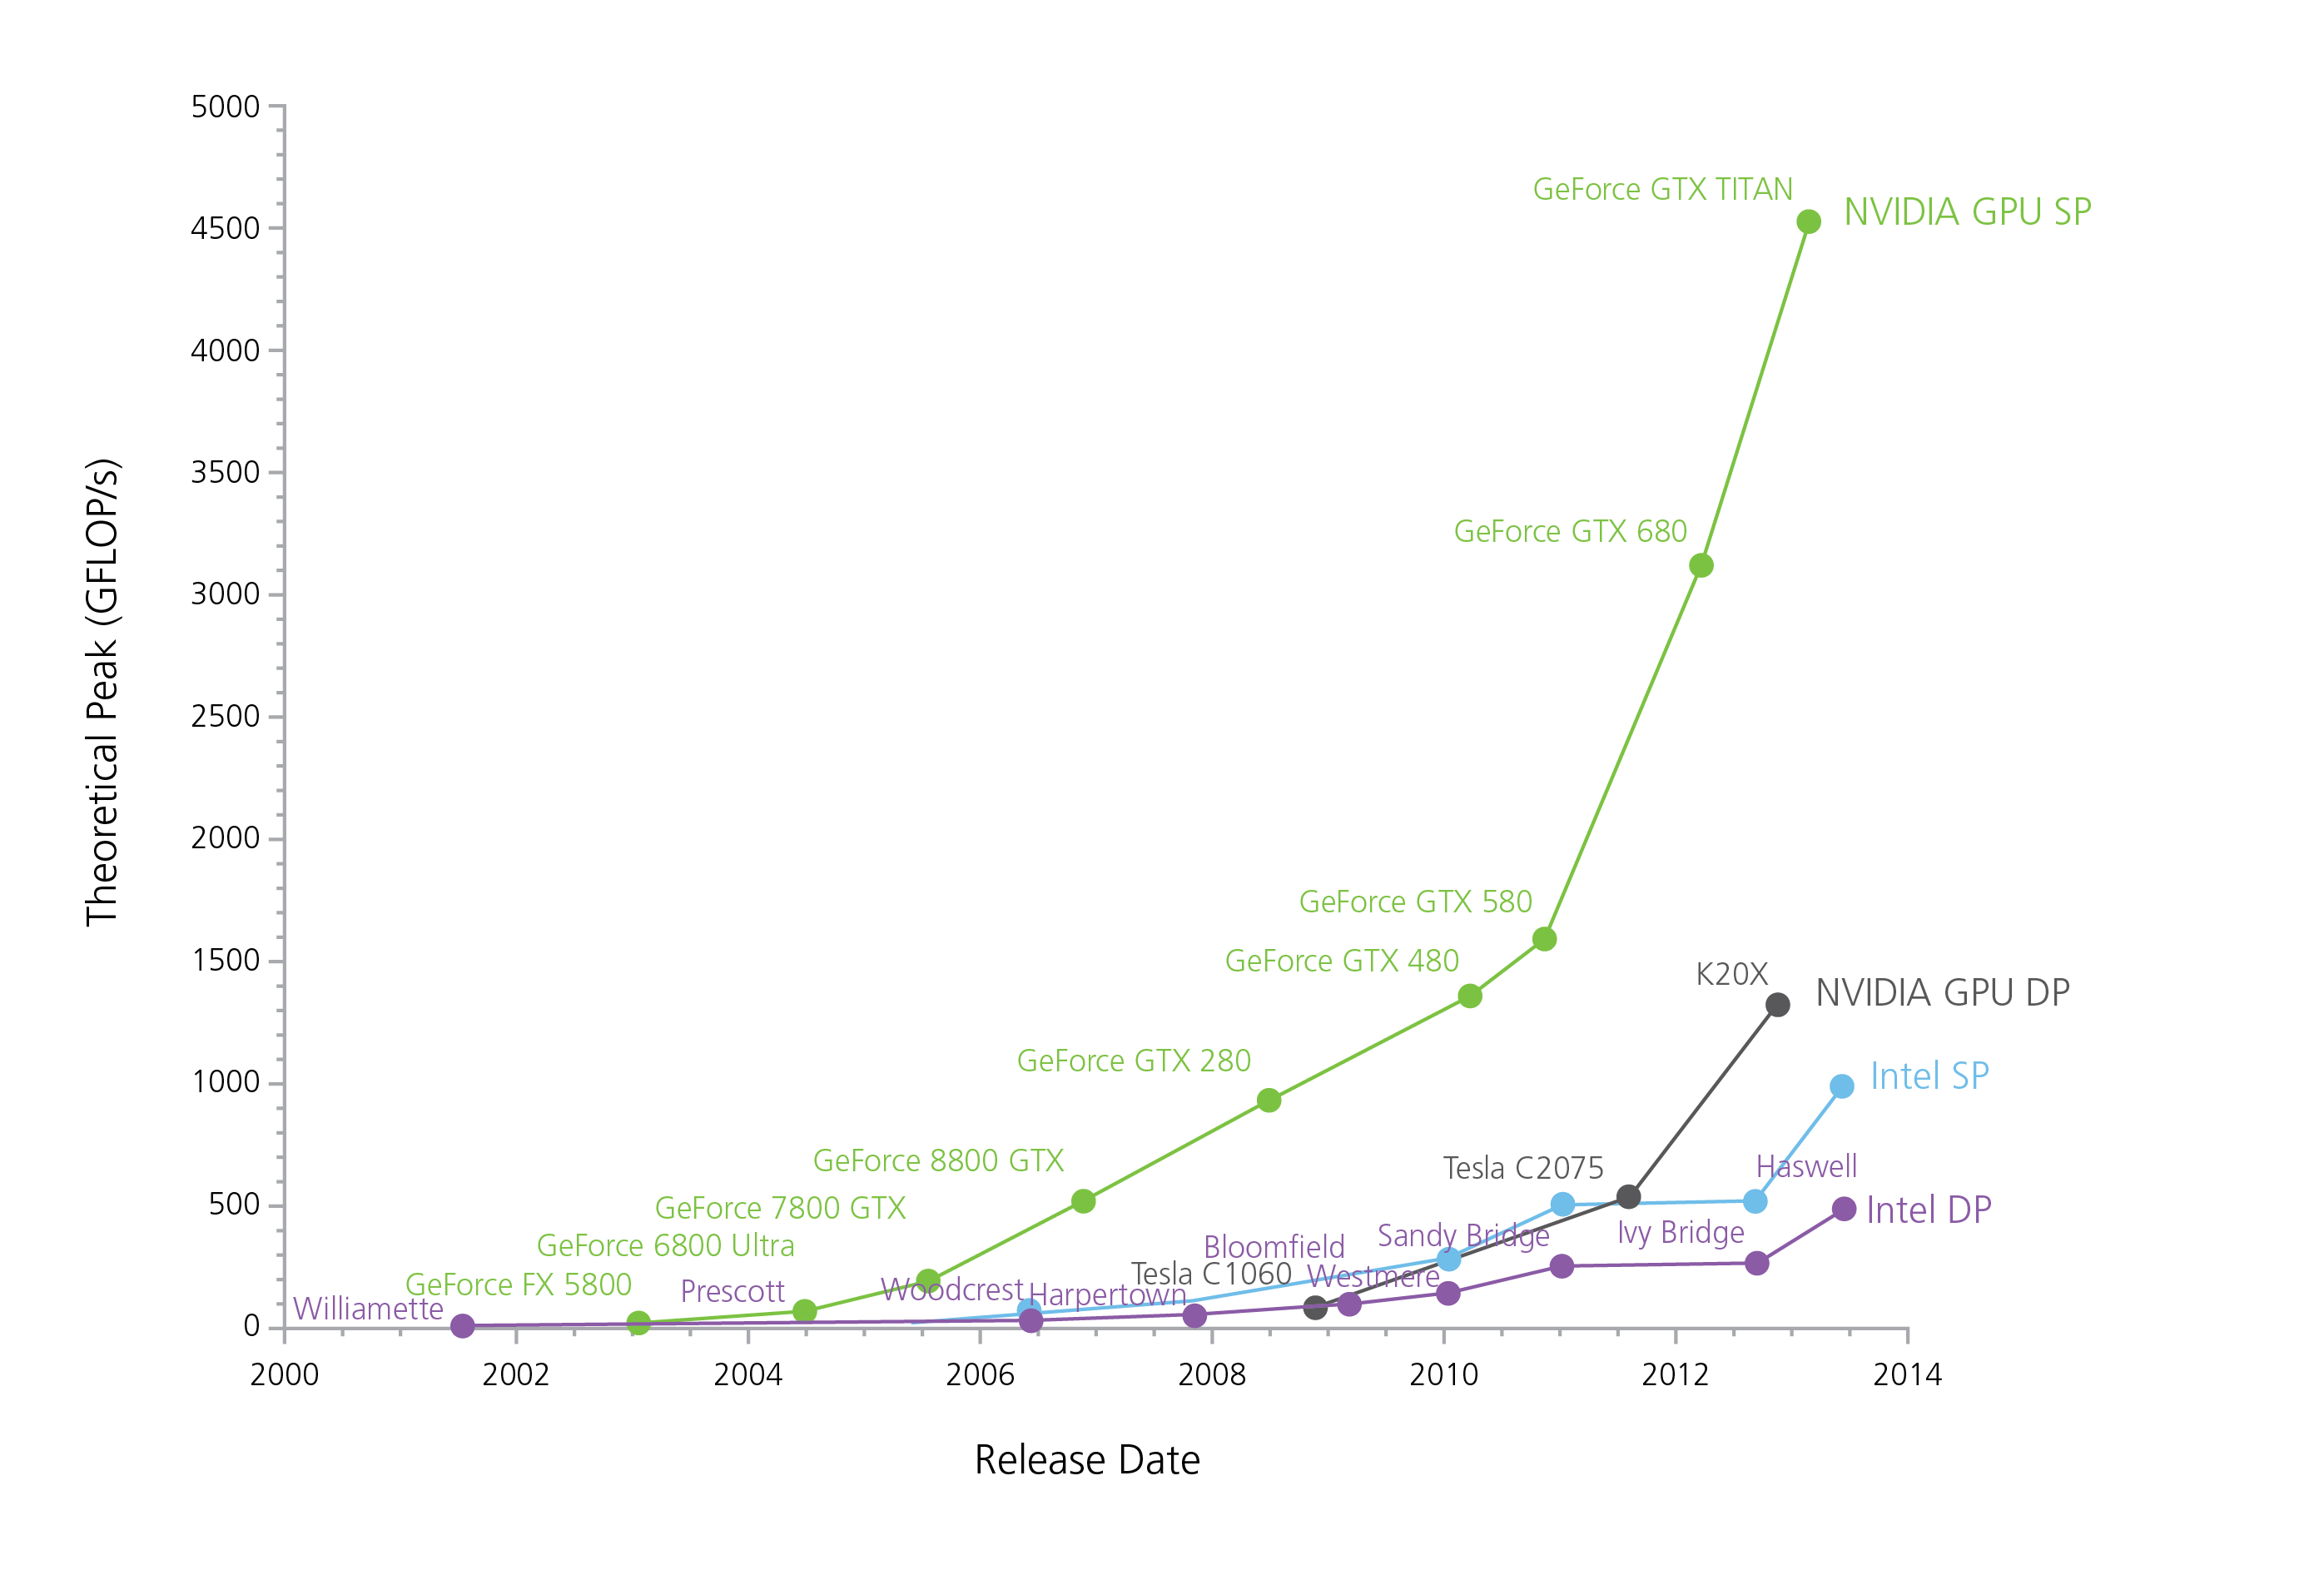
\includegraphics [width=0.9\textwidth]{Introduction/Figs/GPUstats.png}
    \caption{Performance comparison of GPU's over time. \cite{michaelGalloy}}
    \label{fig:GPUStats}
\end{figure}

Higher level skeleton programming libraries have also been developed, which aims to make the parallelization of a problem easier with the use of higher-order functions, skeletons. One such library is SkePU, which was originally developed by Johan Enmyren and Christoph Kessler at Linköping University \cite{enmyren2010skepu}. The major revision SkePU 2 was designed by August Ernstsson, Lu Li and Christoph Kessler and is today maintained by August Ernstsson. Other alternatives exists such as \textbf{OpenAAC} which is a programming standard developed by Cray, CAPS, Nvidia and PGI \cite{OpenACC}, Nvidia's own template library for CUDA, \textbf{Thrust} \cite{Thrust}, and SYCL, which is is OpenCL's equivalent to Thrust \cite{SYCL}.


%********************************** %Second Section  *************************************
\section{Aim} %Section - 1.2

This paper aims to evaluate different GPGPU frameworks in terms of performance, portability, code complexity and features with less focus on the performance evaluation. A suitable benchmarking algorithm will be implemented in the GPGPU frameworks CUDA, OpenCL and DirectX DirectCompute, as well as an implementation in the higher level skeleton library SkePU. The parallelized implementations will be evaluated against a sequential implementation of the same problem.


%********************************** % Third Section  *************************************
\section{Research questions}  %Section - 1.3 

\begin{itemize}
    \item What is a suitable benchmarking algorithm?
    \item How does a parallel implementation of the algorithm compare to a sequential implementation?
    \item What framework-specific optimization's can be done for the implementation?
    \item How does the frameworks compare in terms of portability, code complexity and performance and features?
\end{itemize}


%********************************** % Fourth Section  *************************************
\section{Delimitations}

The selected algorithm will only be implemented in the discussed frameworks:
\begin{itemize}
    \item CUDA
    \item OpenCL
    \item DirectCompute
\end{itemize}

\noindent aswell as an implementation in SkePU, running OpenCL, CUDA, OpenMP and a sequential backend \cite{enmyren2010skepu}. The selected algorithm will thus not be implemented in other GPGPU frameworks and architectures such as OpenGL's compute shader, or a parallel CPU based implementation using e.g OpenMP or similar frameworks.

Even though other optimization algorithms exists for the N-Body problem, only the Barnes-Hut algorithm will be implemented in this work. The reason for this is because the thesis will not focus on evaluating the performance of the frameworks when running the selected algorithm, but on the comparison between frameworks in terms of portability, code complexity and features, which multiple optimization techniques implementations won't contribute to. Furthermore to give the implementation a fair comparison, the tree-structure used in Barnes-Hut will be a sequential implementation and will be performed on the host.

\section{Related work}
This section describes previous research on the subject, both in terms of performance comparisons, but also what previous work and research has been done in terms of the N-Body problem as well as comparisons between the discussed frameworks.


\subsection{Framework comparison} \label{subsec:frameworkComparison}
In 2016 a similar master thesis was performed by T. Sörman where the frameworks CUDA, OpenCL, DirectCompute and OpenGL was compared as well as how the GPGPU implementations performed compared to an multithreaded implementation in OpenMP. \cite{Torbjorn}. Also performed at MindRoad AB, the thesis compares the different frameworks primarily in terms of performance, unlike this thesis which puts more focus on the portability, code complexity and features of the different frameworks. This work will also evaluate the skeleton programming framework SkePU which was not included in Sörmans research \cite{enmyren2010skepu}. 

The algorithm Sörman evaluated is a parallel implementation of the Fast Fourier Transform (FFT), and the result showed that the fastest framework, CUDA, was twice as fast as the slowest, OpenCL, and that the compute shader based frameworks OpenGL and DirectX, are competitive with both CUDA and DirectX in terms of performance.

A lot of previous research has been abducted on the subject of comparing the performance between CUDA and OpenCL. K. Karimi et. al. performed an performance comparison between the two frameworks which showed similar results to Sörmans comparison \cite{karimi2010performance}. Although the performance gap was more subtle in Karimi. et. al. work, the result still showed that CUDA was faster than OpenCL. 

Another more comprehensive study between the two frameworks was abducted by J. Fang et. al. \cite{fang2011comprehensive}. The conducted study compares OpenCL and CUDA in terms of performance when a wide variety of benchmarking algorithms, such as graph traversal, reduction as well the N-Body problem and more, are executed in the two frameworks. Unlike the previously discussed comparisons, the result showed that under a fair comparison the performance difference between the two frameworks was very subtle. 

Another comparison study between CUDA, OpenCL and OpenGL, as well as a CPU multicore implementation that uses OpenMP has been made by R. S. Oliveira et. al. \cite{oliveira2011comparing}. The comparison was based of implementations of the Cardiac Monodomain Equations, and the results showed that the OpenGL approach was the fastest with a speedup of 446 compared to the multicore implementation for a solution of a non-linear system of ordinary differential equations (ODEs). CUDA was the fastest for a numerical solution of parabolic partial diffential equations (PDEs) with a speedup of 8. OpenCL was the slowest for solving the PDEs and as fast as CUDA for solving ODEs.


Although a lot of research comparing CUDA and OpenCL have been made, very little comparisons has been made comparing SkePU with other frameworks. C. Kessler et. al. performed a comparison between SkePU running various backends, to various other implementations: \cite{enmyren2010skepu}
\begin{itemize}
    \item \textbf{ls-seq-def:} The default sequential implementation in LibSolve
    \item \textbf{ls-seq-A:} A slightly optimized variant of ls-seq-def.
    \item \textbf{ls-shm-def:} The default shared memory implementation in LibSolve. It uses pthreads and were run with 8 threads, one for each core of the benchmarking computer.
    \item \textbf{ls-shm-A:} A slightly optimized variant of ls-shm-def. It also uses pthreads and were run with 8 threads.
    \item \textbf{skepu-CL:} SkePU port of ls-seq-def using OpenCL as backend and running on one Tesla C1060 GPU.
    \item \textbf{skepu-CL-multi:} SkePU port of ls-seq-def using OpenCL as backend and running on two Tesla C1060 GPU.
    \item \textbf{skepu-CU:} SkePU port of ls-seq-def using CUDA as backend and running on one Tesla C1060 GPU.
    \item \textbf{skepu-OMP:} SkePU port of ls-seq-def using OpenMP as backend and utilizing 8 threads. 
    \item \textbf{skepu-CPU:} SkePU port of ls-seq-def using the default CPU backend.
    \item \textbf{CU-hand:} A ”hand” implemented CUDA variant. It is similar to the SkePU ports however no SkePU code was utilized. Instead CUBLAS functions were used where applicable and some hand made kernels.

\end{itemize}
\noindent The result of this comparison can be seen in figure \ref{fig:SkepuComparisonODE}. 
C. Kessler et. al. paper also included a comparison between an implementation of a dot product, with SkePU running on different backends compared to CUBLAS, an NVidia CUDA implementation of a dot product calculation. As can be seen in figure \ref{fig:SkepuComparisonDOT}, the results showed that the performance of the SkePU CUDA version is very similar to that of the CUBLAS version.

\begin{figure}[!htbp]
    \centering
    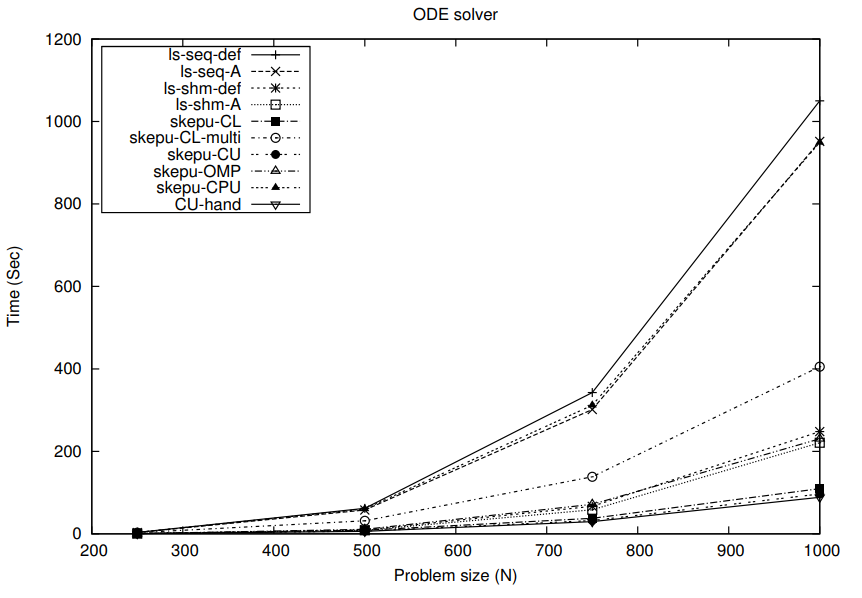
\includegraphics[width=\textwidth]{Introduction/Figs/SkePUComparison.png}
    \caption{SkePU times for running different LibSolve solvers for N =250,500,750 and 1000 with the BRUSS2D-MIX problem. \cite{enmyren2010skepu}}
    \label{fig:SkepuComparisonODE}
\end{figure}

\begin{figure}[!htbp]
    \centering
    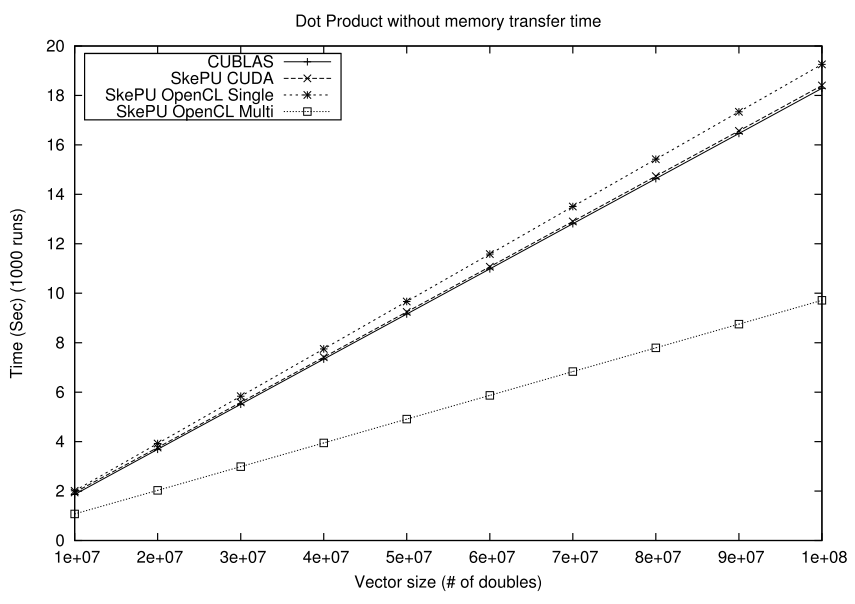
\includegraphics[width=\textwidth]{Introduction/Figs/SkePUComparisonDOT.png}
    \caption{Time for 1000 runs of dot product calculation without host-to-device memory transfer time. \cite{enmyren2010skepu}}
    \label{fig:SkepuComparisonDOT}
\end{figure}


\subsection{N-Body with Barnes-Hut}
The N-Body problem is a common problem, and a lot of previous work has been done regarding the N-Body problem. In the book GPU Gems 3, L. Nyland et. al. at NVIDIA corporation describes a parallel CUDA implementation of the N-Body used to generate an astrophysical simulation \cite{nyland2007fast}. The implementation is done in CUDA, and describes various methods how the CUDA implementation can be optimized with the use of e.g. shared memory, loop-unrolling and coalesced memory accesses. The result of the performance can be seen in figure \ref{fig:GPUGemsNBodyPerformance}. The implementation described in this article does not use the Barnes-Hut algorithm to further speed up the simulation, but instead use what Nyland et. al. call \textit{all-pairs}, meaning that all N-bodies are compared to all other, resulting in the base implementation further described in section \ref{subsec:TheoryNBody}. 

\begin{figure}[!htpb]
    \centering
    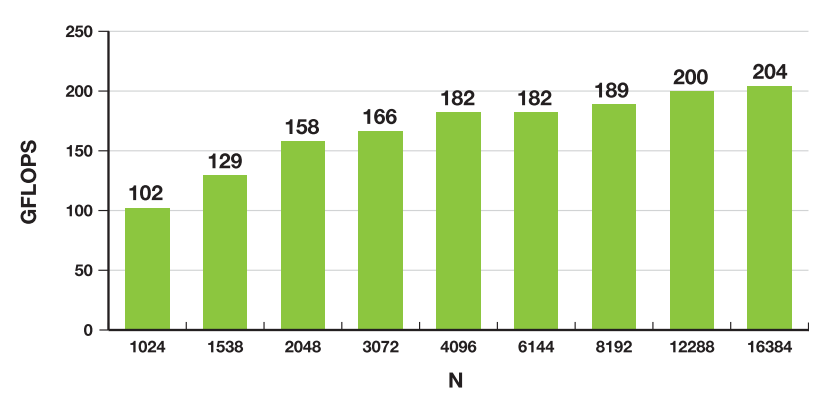
\includegraphics[width=\textwidth]{Introduction/Figs/GPUGemsNBodyComparison.png}
    \caption{N-Body performance increase as N grows. \cite{nyland2007fast}}
    \label{fig:GPUGemsNBodyPerformance}
\end{figure}

Another paper describing the N-body problem, and how it can be applied to astrophysical simulations is S. J. Aarseth's paper \cite{aarseth2003gravitational}. Aarseth's work describes the historical development of the N-body problem, as well as a detailed description of the physical properties of the N-Body problem.


M. Burtscher et. al. made an implementation of the N-Body problem in CUDA with the Barnes-Hut optimization \cite{burtscher2011efficient}. With focus on optimizing the implementation, most of the algorithm was performed on the GPU, resulting in minimal overhead of copying data back and forth between the host and device. M. Burtscher et. al. divided the implementation into six main steps, all performed on the GPU:
\begin{enumerate}
    \item Compute bounding box around all bodies
    \item Build hierarchical decomposition by inserting each body into octree
    \item Summarize body information in each internal octree node
    \item Approximately sort the bodies by spatial distance
    \item Compute forces acting on each body with help of octree
    \item Update body positions and velocities
\end{enumerate}

\noindent The implementation was only done in CUDA and the paper focuses how the implementation is optimized by e.g maximizing coalescing, minimize GPU/CPU data transfer, loop-unrolling etc. The resulting performance of the simulation when run in a sequential CPU implementation, all-pairs parallel implementation as well as a parallel Barnes-Hut implementation can be seen in figure \ref{fig:BurtscherResults}.

\begin{figure}[!htpb]
    \centering
    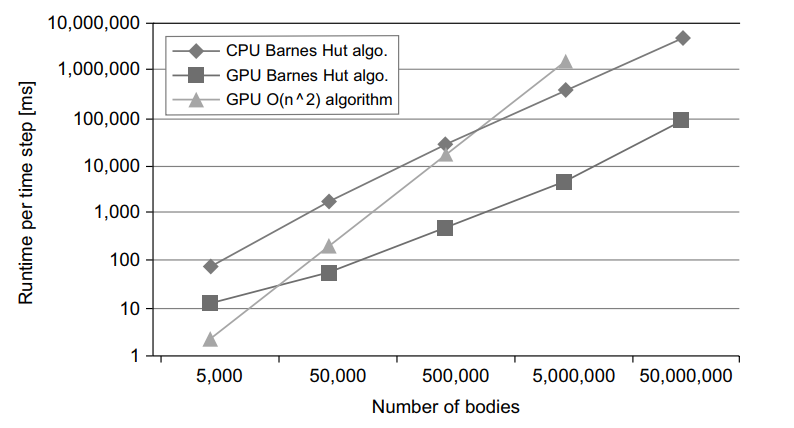
\includegraphics[width=\textwidth]{Introduction/Figs/CPUvsGPUn2vsBarnesHut.png}
    \caption{Runtime per simulated step in M. Burtscher et. al. CUDA implementation of the N-Body problem. \cite{burtscher2011efficient}}
    \label{fig:BurtscherResults}
\end{figure}

\nomenclature[z-ODE]{ODE}{Ordinary Differential Equations}
\nomenclature[z-PDE]{PDE}{Partial Differential Equations}
\nomenclature[z-FFT]{FFT}{Fast Fourier Transform}
\nomenclature[z-OPC]{OpenCL}{Open Computing Language}
\nomenclature[z-CPU]{CPU}{Central Processing Unit}
\nomenclature[z-GPU]{GPU}{Graphics Processing Units}
\nomenclature[z-GPG]{GPGPU}{General-purpose Computing on Graphics Processing Units}
\nomenclature[z-ILP]{ILP}{Instruction Level Parallelism}